
    \documentclass{standalone}
    \usepackage{tikz}

    \begin{document}

    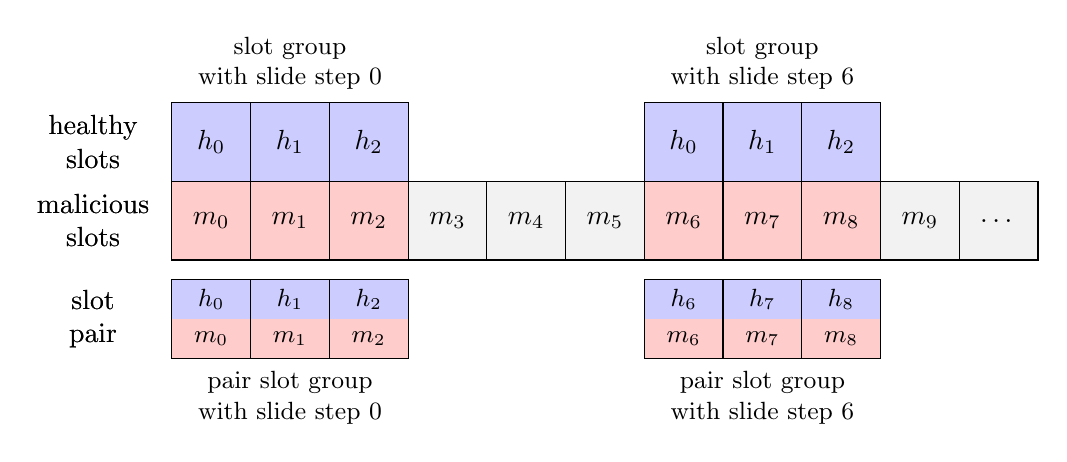
\begin{tikzpicture}

    
\node [align=center, font=\small] at (7.5, 2.5) {slot group\\with slide step 6};
\node [align=center, font=\small] at (7.5, -1.75) {pair slot group\\with slide step 6};
\node[anchor=center,align=center] at (-1, 0.5) {malicious\\slots} ;
\node[anchor=center,align=center] at (-1, -0.75) {slot\\pair} ;
\draw[fill=red!20] (0, 0) rectangle ++(1, 1);
\node[] at (0.5, 0.5) {$m_{0}$};
\node[minimum width=1cm,minimum height=0.5cm,inner ysep=0,font=\small,fill=blue!20] at (0.5, -0.5) {$h_{0}$};
\node[minimum width=1cm,minimum height=0.5cm,inner ysep=0,font=\small,fill=red!20] at (0.5, -1) {$m_{0}$};
\draw (0, -1.25) rectangle ++ (1, 1);
\draw[fill=red!20] (1, 0) rectangle ++(1, 1);
\node[] at (1.5, 0.5) {$m_{1}$};
\node[minimum width=1cm,minimum height=0.5cm,inner ysep=0,font=\small,fill=blue!20] at (1.5, -0.5) {$h_{1}$};
\node[minimum width=1cm,minimum height=0.5cm,inner ysep=0,font=\small,fill=red!20] at (1.5, -1) {$m_{1}$};
\draw (1, -1.25) rectangle ++ (1, 1);
\draw[fill=red!20] (2, 0) rectangle ++(1, 1);
\node[] at (2.5, 0.5) {$m_{2}$};
\node[minimum width=1cm,minimum height=0.5cm,inner ysep=0,font=\small,fill=blue!20] at (2.5, -0.5) {$h_{2}$};
\node[minimum width=1cm,minimum height=0.5cm,inner ysep=0,font=\small,fill=red!20] at (2.5, -1) {$m_{2}$};
\draw (2, -1.25) rectangle ++ (1, 1);
\draw[fill=gray!10] (3, 0) rectangle ++(1, 1);
\node[] at (3.5, 0.5) {$m_{3}$};
\draw[fill=gray!10] (4, 0) rectangle ++(1, 1);
\node[] at (4.5, 0.5) {$m_{4}$};
\draw[fill=gray!10] (5, 0) rectangle ++(1, 1);
\node[] at (5.5, 0.5) {$m_{5}$};
\draw[fill=red!20] (6, 0) rectangle ++(1, 1);
\node[] at (6.5, 0.5) {$m_{6}$};
\node[minimum width=1cm,minimum height=0.5cm,inner ysep=0,font=\small,fill=blue!20] at (6.5, -0.5) {$h_{6}$};
\node[minimum width=1cm,minimum height=0.5cm,inner ysep=0,font=\small,fill=red!20] at (6.5, -1) {$m_{6}$};
\draw (6, -1.25) rectangle ++ (1, 1);
\draw[fill=red!20] (7, 0) rectangle ++(1, 1);
\node[] at (7.5, 0.5) {$m_{7}$};
\node[minimum width=1cm,minimum height=0.5cm,inner ysep=0,font=\small,fill=blue!20] at (7.5, -0.5) {$h_{7}$};
\node[minimum width=1cm,minimum height=0.5cm,inner ysep=0,font=\small,fill=red!20] at (7.5, -1) {$m_{7}$};
\draw (7, -1.25) rectangle ++ (1, 1);
\draw[fill=red!20] (8, 0) rectangle ++(1, 1);
\node[] at (8.5, 0.5) {$m_{8}$};
\node[minimum width=1cm,minimum height=0.5cm,inner ysep=0,font=\small,fill=blue!20] at (8.5, -0.5) {$h_{8}$};
\node[minimum width=1cm,minimum height=0.5cm,inner ysep=0,font=\small,fill=red!20] at (8.5, -1) {$m_{8}$};
\draw (8, -1.25) rectangle ++ (1, 1);
\draw[fill=gray!10] (9, 0) rectangle ++(1, 1);
\node[] at (9.5, 0.5) {$m_{9}$};
\draw[fill=gray!10] (10, 0) rectangle ++(1, 1);
\node[] at (10.5, 0.5) {\dots};
\node[anchor=center,align=center] at (-1, 1.5) {healthy\\slots};
\draw[fill=blue!20] (6, 1) rectangle ++(1, 1);
\node[] at (6.5, 1.5) {$h_{0}$};
\draw[fill=blue!20] (7, 1) rectangle ++(1, 1);
\node[] at (7.5, 1.5) {$h_{1}$};
\draw[fill=blue!20] (8, 1) rectangle ++(1, 1);
\node[] at (8.5, 1.5) {$h_{2}$};
\node [align=center, font=\small] at (1.5, 2.5) {slot group\\with slide step 0};
\node [align=center, font=\small] at (1.5, -1.75) {pair slot group\\with slide step 0};
\node[anchor=center,align=center] at (-1, 0.5) {malicious\\slots} ;
\node[anchor=center,align=center] at (-1, -0.75) {slot\\pair} ;
\draw[fill=red!20] (0, 0) rectangle ++(1, 1);
\node[] at (0.5, 0.5) {$m_{0}$};
\node[minimum width=1cm,minimum height=0.5cm,inner ysep=0,font=\small,fill=blue!20] at (0.5, -0.5) {$h_{0}$};
\node[minimum width=1cm,minimum height=0.5cm,inner ysep=0,font=\small,fill=red!20] at (0.5, -1) {$m_{0}$};
\draw (0, -1.25) rectangle ++ (1, 1);
\draw[fill=red!20] (1, 0) rectangle ++(1, 1);
\node[] at (1.5, 0.5) {$m_{1}$};
\node[minimum width=1cm,minimum height=0.5cm,inner ysep=0,font=\small,fill=blue!20] at (1.5, -0.5) {$h_{1}$};
\node[minimum width=1cm,minimum height=0.5cm,inner ysep=0,font=\small,fill=red!20] at (1.5, -1) {$m_{1}$};
\draw (1, -1.25) rectangle ++ (1, 1);
\draw[fill=red!20] (2, 0) rectangle ++(1, 1);
\node[] at (2.5, 0.5) {$m_{2}$};
\node[minimum width=1cm,minimum height=0.5cm,inner ysep=0,font=\small,fill=blue!20] at (2.5, -0.5) {$h_{2}$};
\node[minimum width=1cm,minimum height=0.5cm,inner ysep=0,font=\small,fill=red!20] at (2.5, -1) {$m_{2}$};
\draw (2, -1.25) rectangle ++ (1, 1);
\draw[fill=gray!10] (3, 0) rectangle ++(1, 1);
\node[] at (3.5, 0.5) {$m_{3}$};
\draw[fill=gray!10] (4, 0) rectangle ++(1, 1);
\node[] at (4.5, 0.5) {$m_{4}$};
\draw[fill=gray!10] (5, 0) rectangle ++(1, 1);
\node[] at (5.5, 0.5) {$m_{5}$};
\draw[fill=red!20] (6, 0) rectangle ++(1, 1);
\node[] at (6.5, 0.5) {$m_{6}$};
\node[minimum width=1cm,minimum height=0.5cm,inner ysep=0,font=\small,fill=blue!20] at (6.5, -0.5) {$h_{6}$};
\node[minimum width=1cm,minimum height=0.5cm,inner ysep=0,font=\small,fill=red!20] at (6.5, -1) {$m_{6}$};
\draw (6, -1.25) rectangle ++ (1, 1);
\draw[fill=red!20] (7, 0) rectangle ++(1, 1);
\node[] at (7.5, 0.5) {$m_{7}$};
\node[minimum width=1cm,minimum height=0.5cm,inner ysep=0,font=\small,fill=blue!20] at (7.5, -0.5) {$h_{7}$};
\node[minimum width=1cm,minimum height=0.5cm,inner ysep=0,font=\small,fill=red!20] at (7.5, -1) {$m_{7}$};
\draw (7, -1.25) rectangle ++ (1, 1);
\draw[fill=red!20] (8, 0) rectangle ++(1, 1);
\node[] at (8.5, 0.5) {$m_{8}$};
\node[minimum width=1cm,minimum height=0.5cm,inner ysep=0,font=\small,fill=blue!20] at (8.5, -0.5) {$h_{8}$};
\node[minimum width=1cm,minimum height=0.5cm,inner ysep=0,font=\small,fill=red!20] at (8.5, -1) {$m_{8}$};
\draw (8, -1.25) rectangle ++ (1, 1);
\draw[fill=gray!10] (9, 0) rectangle ++(1, 1);
\node[] at (9.5, 0.5) {$m_{9}$};
\draw[fill=gray!10] (10, 0) rectangle ++(1, 1);
\node[] at (10.5, 0.5) {\dots};
\node[anchor=center,align=center] at (-1, 1.5) {healthy\\slots};
\draw[fill=blue!20] (0, 1) rectangle ++(1, 1);
\node[] at (0.5, 1.5) {$h_{0}$};
\draw[fill=blue!20] (1, 1) rectangle ++(1, 1);
\node[] at (1.5, 1.5) {$h_{1}$};
\draw[fill=blue!20] (2, 1) rectangle ++(1, 1);
\node[] at (2.5, 1.5) {$h_{2}$};


    \end{tikzpicture}

    \end{document}

    
